\documentclass{cshwk}

\title{Principles of Database Systems\\Assignment \#2 - Relation Model}
\begin{document}

\maketitle

\section{Class Assignment}

Create 5 tables that show in slides all \texttt{PRIMARY KEY} and \texttt{FOREIGN KEY} relationships. Also, insert example data that is displayed in the slides. The schema is shown in Fig.~\ref{fig:schema}.

\begin{figure}[H]
    \centering
    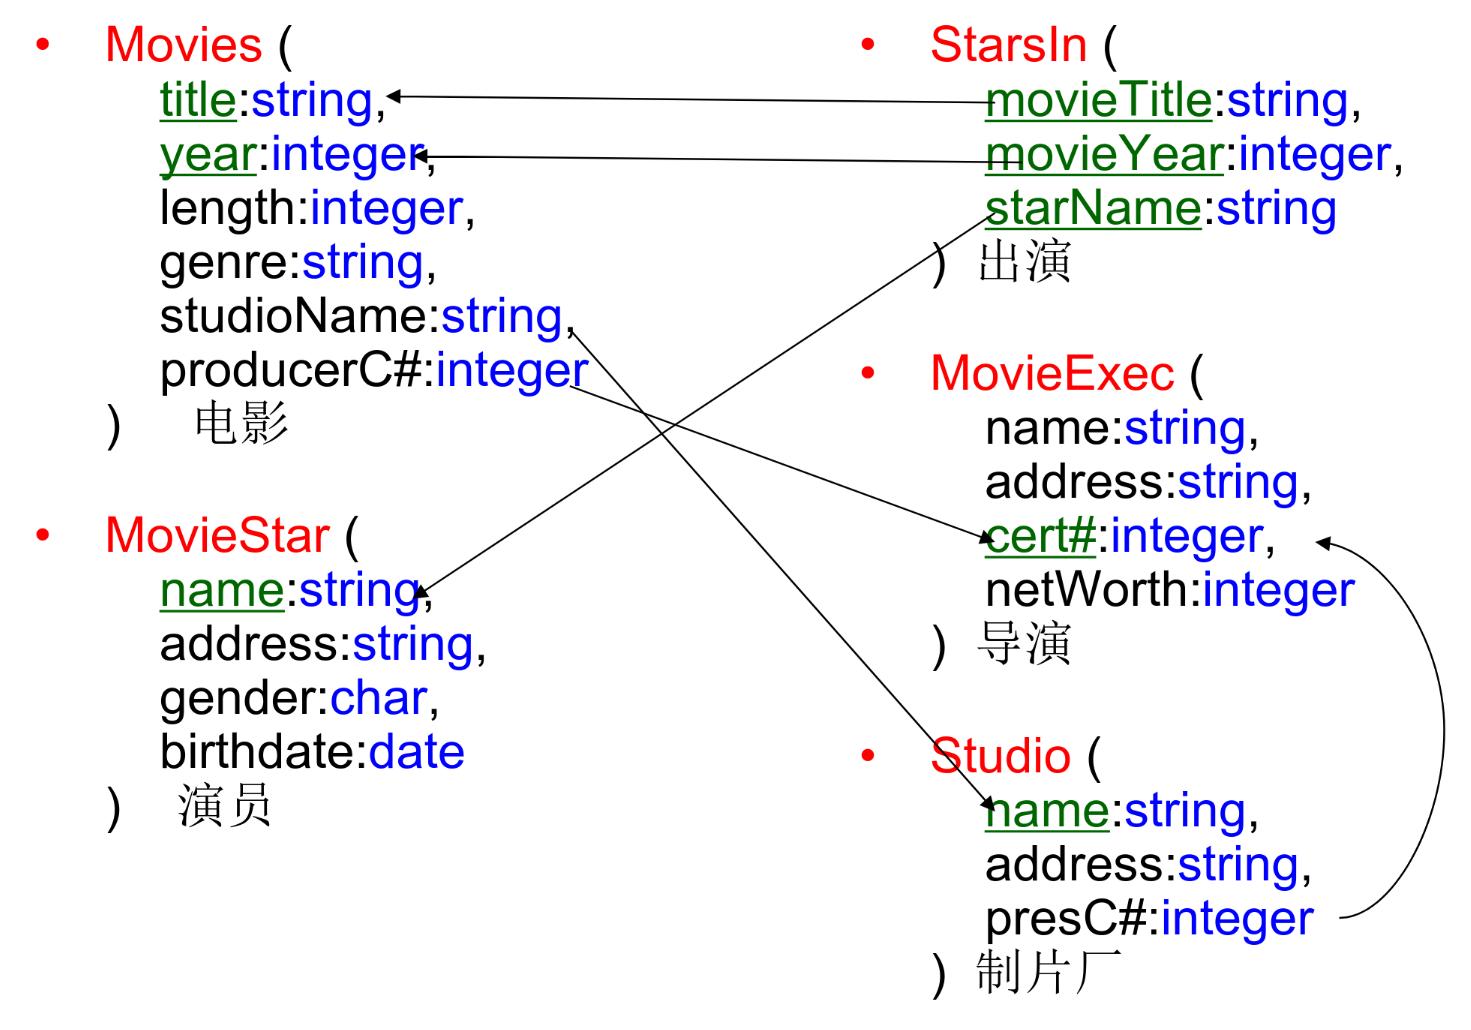
\includegraphics[width=0.6\textwidth]{hw2-2.png}
    \caption{Example Database Schema}
    \label{fig:schema}
\end{figure}

\subsection*{Solutions}

First, we need to identify the \texttt{PRIMARY KEY} and \texttt{FOREIGN KEY}. The \texttt{PRIMARY KEY}s are:
\begin{enumerate}
    \item \texttt{Movies}: \texttt{title + year}
    \item \texttt{MovieStar}: \texttt{name}
    \item \texttt{StarsIn}: \texttt{movieTitle + movieYear + starName}
    \item \texttt{MovieExec}: \texttt{cert\#}
    \item \texttt{Studio}: \texttt{name}
\end{enumerate}

\noindent The \texttt{FOREIGN KEY} relationships are:
\begin{enumerate}
    \item \texttt{Movies.studioName} references \texttt{Studio.name}
    \item \texttt{Movies.producerC\#} references \texttt{MovieExec.cert\#}
    \item \texttt{StarsIn.movieTitle} and \texttt{StarsIn.movieYear} reference \texttt{Movies.title} and \texttt{Movies.year}
    \item \texttt{StarsIn.starName} references \texttt{MovieStar.name}
    \item \texttt{Studio.presC\#} references \texttt{MovieExec.cert\#}
\end{enumerate}

\noindent The SQL table definitions with \texttt{PRIMARY KEY} and \texttt{FOREIGN KEY} constraints are as follows:

\subsection*{SQL Table Definitions}

\begin{verbatim}
    -- 1. Create MovieExec first (no dependencies)
    CREATE TABLE MovieExec (
        name VARCHAR(255),
        address VARCHAR(255),
        "cert#" INT,
        netWorth DECIMAL(10, 2),
        PRIMARY KEY ("cert#")
    );
    
    -- 2. Create Studio (depends on MovieExec)
    CREATE TABLE Studio (
        name VARCHAR(255),
        address VARCHAR(255),
        "presC#" INT,
        PRIMARY KEY (name),
        FOREIGN KEY ("presC#") REFERENCES MovieExec("cert#")
    );
    
    -- 3. Create MovieStar (no dependencies)
    CREATE TABLE MovieStar (
        name VARCHAR(255),
        address VARCHAR(255),
        gender CHAR(1),
        birthdate DATE,
        PRIMARY KEY (name)
    );
    
    -- 4. Create Movies (depends on Studio and MovieExec)
    CREATE TABLE Movies (
        title VARCHAR(255),
        year INT,
        length INT,
        genre VARCHAR(50),
        studioName VARCHAR(255),
        "producerC#" INT,
        PRIMARY KEY (title, year),
        FOREIGN KEY (studioName) REFERENCES Studio(name),
        FOREIGN KEY ("producerC#") REFERENCES MovieExec("cert#")
    );
    
    -- 5. Create StarsIn (depends on Movies and MovieStar)
    CREATE TABLE StarsIn (
        movieTitle VARCHAR(255),
        movieYear INT,
        starName VARCHAR(255),
        PRIMARY KEY (movieTitle, movieYear, starName),
        FOREIGN KEY (movieTitle, movieYear) REFERENCES Movies(title, year),
        FOREIGN KEY (starName) REFERENCES MovieStar(name)
    );    
\end{verbatim}

\subsection*{Example Data Insertions}

\begin{verbatim}
    -- 1. Insert into MovieExec Table
    INSERT INTO MovieExec (name, address, "cert#", netWorth)
    VALUES ('John Smith', 'Hollywood Blvd, USA', 101, 5000000.00);
    
    -- 2. Insert into Studio Table
    INSERT INTO Studio (name, address, "presC#") 
    VALUES ('Warner Bros', 'California, USA', 101);
    
    -- 3. Insert into MovieStar Table
    INSERT INTO MovieStar (name, address, gender, birthdate)
    VALUES ('Leonardo DiCaprio', 'LA, USA', 'M', '1974-11-11');
    
    -- 4. Insert into Movies Table
    INSERT INTO Movies (title, year, length, genre, studioName, "producerC#")
    VALUES ('Inception', 2010, 148, 'Sci-Fi', 'Warner Bros', 101);
    
    -- 5. Insert into StarsIn Table
    INSERT INTO StarsIn (movieTitle, movieYear, starName)
    VALUES ('Inception', 2010, 'Leonardo DiCaprio');    
\end{verbatim}

This schema demonstrates the relationships between tables, highlighting the \texttt{PRIMARY KEY} and \texttt{FOREIGN KEY} constraints and showing how to insert example data accordingly.

\subsection*{Running in MySQL}

Here we use \texttt{PostgreSQL} as the database, and use \texttt{DataGrip} as the client to run the SQL queries.
The results are shown in Fig.~\ref{fig:table_create_1}-\ref{fig:data_instertions}.
\begin{figure}[H]
    \centering
    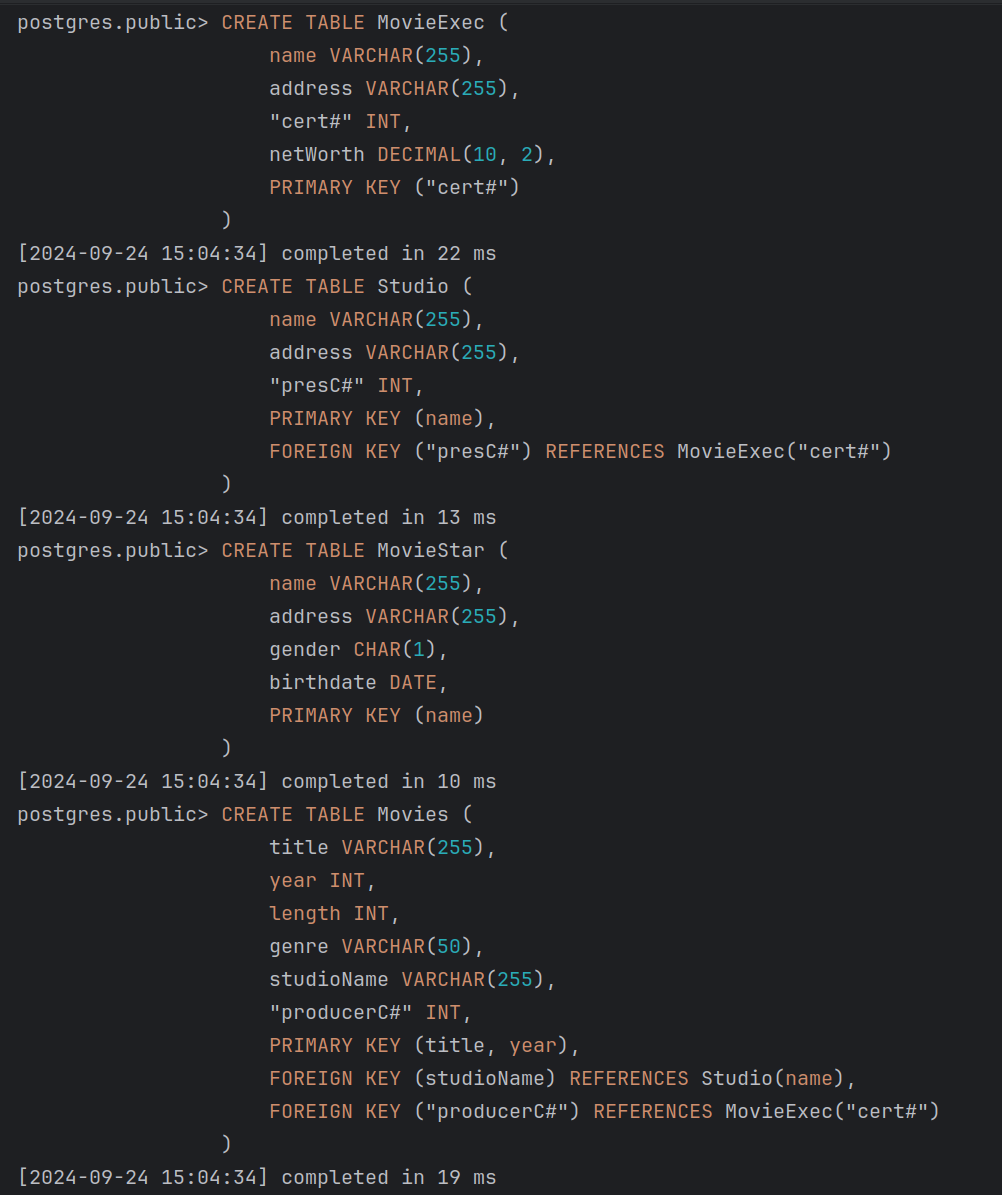
\includegraphics[width=0.8\textwidth]{hw2-3.png}
    \caption{Results of SQL Queries}
    \label{fig:table_create_1}
\end{figure}

\begin{figure}[H]
    \centering
    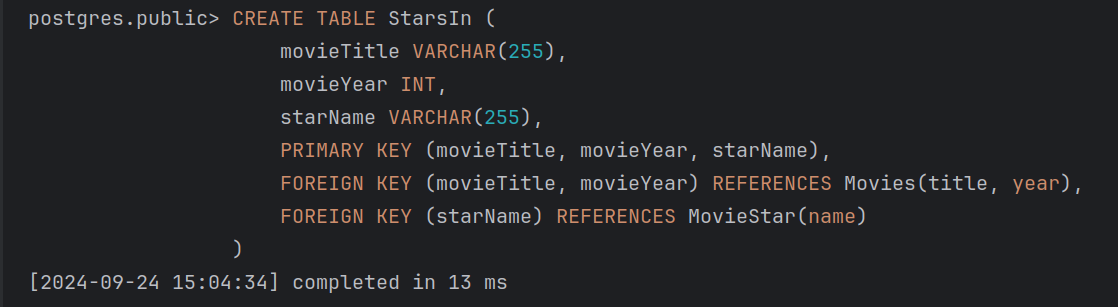
\includegraphics[width=0.8\textwidth]{hw2-4.png}
    \caption{Results of SQL Queries}
    \label{fig:table_create_2}
\end{figure}

\begin{figure}[H]
    \centering
    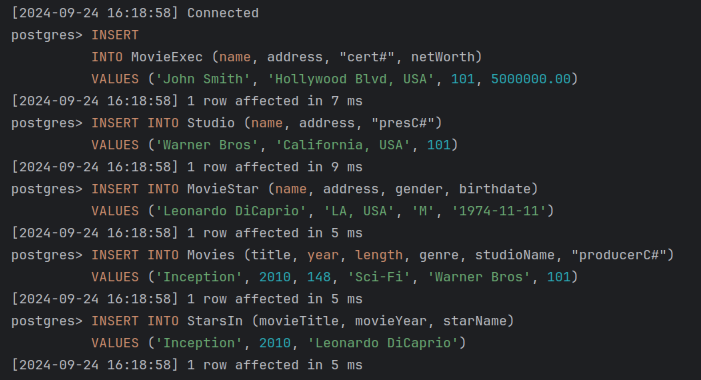
\includegraphics[width=0.8\textwidth]{hw2-5.png}
    \caption{Results of Data Insertions}
    \label{fig:data_instertions}
\end{figure}


\section{Exercise 2.2.1}

In Fig.~\ref{fig:221-fig} are instances of two relations that might constitute
part of a banking database. Indicate the following:
\begin{enumerate}
    \item The attributes of each relation.
    \item The tuples of each relation.
    \item The components of one tuple from each relation.
    \item The relation schema for each relation.
    \item The database schema.
    \item A suitable domain for each attribute.
    \item Another equivalent way to present each relation.
\end{enumerate}

\begin{figure}[H]
    \centering
    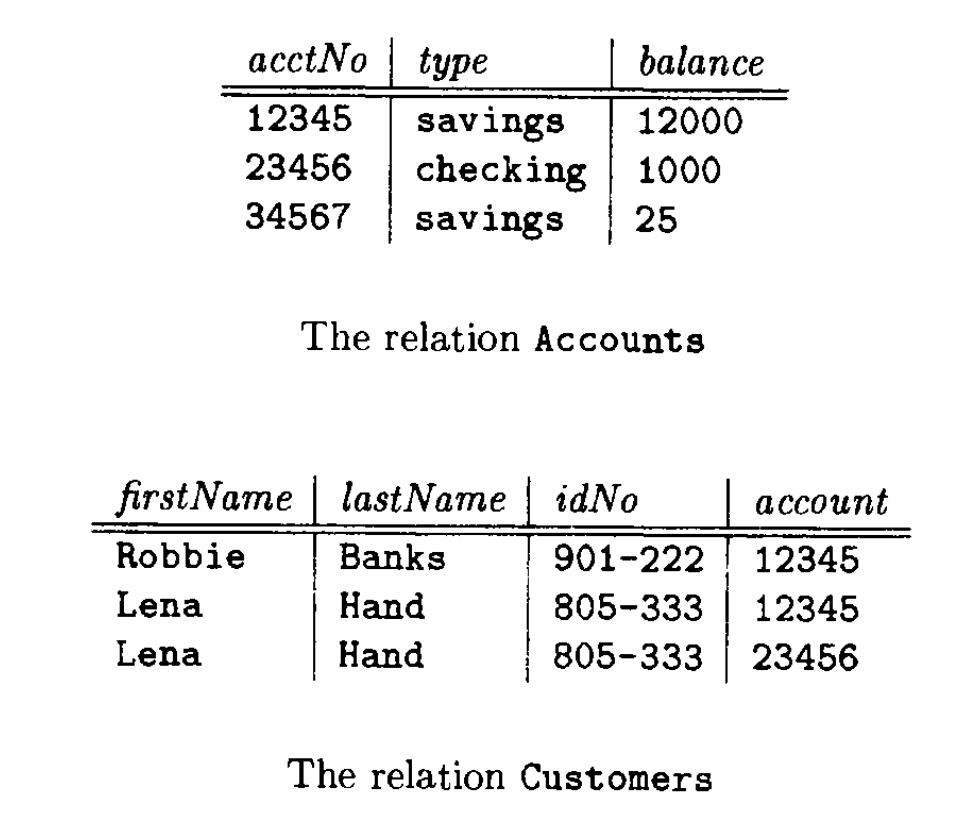
\includegraphics[width=0.5\textwidth]{hw2-1.png}
    \caption{Two relations of a banking database}
    \label{fig:221-fig}
\end{figure}

\subsection*{Solutions:}

\subsubsection*{1. Attributes}
For relation \texttt{Accounts}, the attributes are: \texttt{acctNo}, \texttt{type}, \texttt{balance}.

\noindent For relation \texttt{Customers}, the attributes are: \texttt{firstName}, \texttt{lastName}, \texttt{idNo}, and \texttt{account}.

\subsubsection*{2. Tuples}
For relation \texttt{Accounts}, the tuples are:
\begin{itemize}
    \item \texttt{(12345, savings, 12000)}
    \item \texttt{(23456, checking, 1000)}
    \item \texttt{(34567, savings, 25)}
\end{itemize}

\noindent For relation \texttt{Customers}, the tuples are:
\begin{itemize}
    \item \texttt{(Robbie, Banks, 901-222, 12345)}
    \item \texttt{(Lena, Hand, 805-333, 12345)}
    \item \texttt{(Lena, Hand, 805-333, 23456)}
\end{itemize}

\subsubsection*{3. Components of One Tuple from Each Relation}
For the relation \texttt{Accounts}, one tuple is (12345, savings, 12000).
\begin{itemize}
    \item \texttt{acctNo} = 12345
    \item \texttt{type} = savings
    \item \texttt{balance} = 12000
\end{itemize}

\noindent For the relation \texttt{Customers}, one tuple is (Robbie, Banks, 901-222, 12345).
\begin{itemize}
    \item \texttt{firstName} = Robbie
    \item \texttt{lastName} = Banks
    \item \texttt{idNo} = 901-222
    \item \texttt{account} = 12345
\end{itemize}

\subsubsection*{4. Relation Schema}

The schema for \texttt{Accounts} relation is:
\begin{verbatim}
    Accounts(acctNo, type, balance)
\end{verbatim}

\noindent The schema for \texttt{Customers} relation is:
\begin{verbatim}
    Customers(firstName, lastName, idNo, account)
\end{verbatim}

\subsubsection*{5. Database Schema}

The database schema consists of the following relations:

\begin{verbatim}
    Accounts(
        acctNo: INTEGER,
        type: STRING,
        balance: DECIMAL
    )

    Customers(
        firstName: STRING,
        lastName: STRING,
        idNo: STRING,
        account: INTEGER
    )
\end{verbatim}


\subsubsection*{6. Suitable Domain for Each Attribute}
The suitable domains for the attributes are:
\begin{itemize}
    \item \texttt{acctNo}: integer (e.g., a 5-digit number)
    \item \texttt{type}: string (values like \texttt{"savings"} or \texttt{"checking"})
    \item \texttt{balance}: integer or floating point
    \item \texttt{firstName}: string
    \item \texttt{lastName}: string
    \item \texttt{idNo}: string (in a format like a social security number)
    \item \texttt{account}: integer (corresponds to \texttt{acctNo})
\end{itemize}

\subsubsection*{7. Another Equivalent Way to Present Each Relation}
Another way to represent the \texttt{Accounts} relation is in JSON format:
\begin{verbatim}
[
  {"acctNo": 12345, "type": "savings", "balance": 12000},
  {"acctNo": 23456, "type": "checking", "balance": 1000},
  {"acctNo": 34567, "type": "savings", "balance": 25}
]
\end{verbatim}

\noindent Similarly, for the \texttt{Customers} relation:
\begin{verbatim}
    [
        {
          "firstName": "Robbie",
          "lastName": "Banks",
          "idNo": "901-222",
          "account": 12345
        },
        {
          "firstName": "Lena",
          "lastName": "Hand",
          "idNo": "805-333",
          "account": 12345
        },
        {
          "firstName": "Lena",
          "lastName": "Hand",
          "idNo": "805-333",
          "account": 23456
        }
      ]
\end{verbatim}

\section{Exercise 2.3.1}
In this exercise we introduce one of our running examples of a relational database schema. The database schema consists of four relations, whose schemas are:
\begin{itemize}
    \item \texttt{Product(maker, model, type)}
    \item \texttt{PC(model, speed, ram, hd, price)}
    \item \texttt{Laptop(model, speed, ram, hd, screen, price)}
    \item \texttt{Printer(model, color, type, price)}
\end{itemize}

The \texttt{Product} relation gives the manufacturer, model number and type (PC, laptop, or printer) of various products. We assume for convenience that model numbers are unique over all manufacturers and product types; that assumption is not realistic, and a real database would include a code for the manufacturer as part of the model number. The \texttt{PC} relation gives for each model number that is a PC the speed (of the processor, in gigahertz), the amount of RAM (in megabytes), the size of the hard disk (in gigabytes), and the price. The \texttt{Laptop} relation is similar, except that the screen size (in inches) is also included. The \texttt{Printer} relation records for each printer model whether the printer produces color output (true, if so), the process type (laser or ink-jet, typically), and the price.

\textbf{Write the following declarations:}
\begin{enumerate}
    \item A suitable schema for relation \texttt{Product}.
    \item A suitable schema for relation \texttt{PC}.
    \item A suitable schema for relation \texttt{Laptop}.
    \item A suitable schema for relation \texttt{Printer}.
    \item An alteration to your \texttt{Printer} schema from (4) to delete the attribute \texttt{color}.
    \item An alteration to your \texttt{Laptop} schema from (3) to add the attribute \texttt{od} (optical-disk type, e.g., cd or dvd). Let the default value for this attribute be 'none' if the laptop does not have an optical disk.
\end{enumerate}

\subsection*{Solutions}

\subsubsection*{1. Schema of Relation \texttt{Product}}

\begin{verbatim}
    CREATE TABLE Product (
        maker VARCHAR(255),
        model VARCHAR(255) PRIMARY KEY,
        type VARCHAR(50)
    );    
\end{verbatim}

\subsubsection*{2. Schema of Relation \texttt{PC}}
\begin{verbatim}
    CREATE TABLE PC (
        model VARCHAR(255) PRIMARY KEY,
        speed FLOAT,
        ram INT,
        hd INT,
        price DECIMAL(10, 2),
        FOREIGN KEY (model) REFERENCES Product(model)
    );    
\end{verbatim}

\subsubsection*{3. Schema of Relation \texttt{Laptop}}
\begin{verbatim}
    CREATE TABLE Laptop (
        model VARCHAR(255) PRIMARY KEY,
        speed FLOAT,
        ram INT,
        hd INT,
        screen FLOAT,
        price DECIMAL(10, 2),
        FOREIGN KEY (model) REFERENCES Product(model)
    );
\end{verbatim}

\subsubsection*{4. Schema of Relation \texttt{Printer}}
\begin{verbatim}
    CREATE TABLE Printer (
        model VARCHAR(255) PRIMARY KEY,
        color BOOLEAN,
        type VARCHAR(50),
        price DECIMAL(10, 2),
        FOREIGN KEY (model) REFERENCES Product(model)
    );
\end{verbatim}

\subsubsection*{5. Alter the \texttt{Printer} table to delete the attribute \texttt{color}: }
\begin{verbatim}
    ALTER TABLE Printer DROP COLUMN color;    
\end{verbatim}

\subsubsection*{6. Alter the \texttt{Laptop} table to add the attribute \texttt{od} with default value 'none'}

\begin{verbatim}
    ALTER TABLE Laptop
    ADD COLUMN od VARCHAR(50) DEFAULT 'none';
\end{verbatim}

\section{Exercise 2.3.2}
This exercise introduces another running example, concerning World War II capital ships. It involves the following relations:
\begin{itemize}
    \item \texttt{Classes(class, type, country, numGuns, bore, displacement)}
    \item \texttt{Ships(name, class, launched)}
    \item \texttt{Battles(name, date)}
    \item \texttt{Outcomes(ship, battle, result)}
\end{itemize}
Ships are built in "classes" from the same design, and the class is usually named for the first ship of that class. The relation \texttt{Classes} records the name of the class, the type ( 'bb' for battleship or 'be' for battlecruiser), the country that built the ship, the number of main guns, the bore (diameter of the gun barrel, in inches) of the main guns, and the displacement (weight, in tons). Relation \texttt{Ships} records the name of the ship, the name of its class, and the year in which the ship was launched. Relation \texttt{Battles} gives the name and date of battles involving these ships, and relation \texttt{Outcomes} gives the result (sunk, damaged, or ok) for each ship in each battle.

\textbf{Write the following declarations:}
\begin{enumerate}
    \item A suitable schema for relation \texttt{Classes}.
    \item A suitable schema for relation \texttt{Ships}.
    \item A suitable schema for relation \texttt{Battles}.
    \item A suitable schema for relation \texttt{Outcomes}.
    \item An alteration to your \texttt{Classes} relation from (a) to delete the attribute \texttt{bore}.
    \item An alteration to your \texttt{Ships} relation from (b) to include the attribute \texttt{yard} giving the shipyard where the ship was built.
\end{enumerate}

\subsection*{Solutions}

\subsubsection*{1. Schema for Relation \texttt{Classes}:}
\begin{verbatim}
    CREATE TABLE Classes (
        class VARCHAR(50) PRIMARY KEY,
        type CHAR(2) CHECK (type IN ('bb', 'be')),
        country VARCHAR(50),
        numGuns INT,
        displacement FLOAT
    );    
\end{verbatim}

\subsubsection*{2. Schema for Relation \texttt{Ships}}
\begin{verbatim}
    CREATE TABLE Ships (
        name VARCHAR(50) PRIMARY KEY,
        class VARCHAR(50),
        launched YEAR,
        FOREIGN KEY (class) REFERENCES Classes(class)
    );    
\end{verbatim}


\subsubsection*{3. Schema for Relation \texttt{Battles}}
\begin{verbatim}
    CREATE TABLE Battles (
        name VARCHAR(50) PRIMARY KEY,
        date DATE
    );    
\end{verbatim}

\subsubsection*{4. Schema for Relation \texttt{Outcomes}}

\begin{verbatim}
    CREATE TABLE Outcomes (
        ship VARCHAR(50),
        battle VARCHAR(50),
        result CHAR(3) CHECK (result IN ('sunk', 'dam', 'ok')),
        PRIMARY KEY (ship, battle),
        FOREIGN KEY (ship) REFERENCES Ships(name),
        FOREIGN KEY (battle) REFERENCES Battles(name)
    );    
\end{verbatim}

\subsubsection*{5. Alteration to \texttt{Classes} to delete the attribute \texttt{bore}:}

\begin{verbatim}
    ALTER TABLE Classes
    DROP COLUMN bore;    
\end{verbatim}

\subsubsection*{6. Alteration to \texttt{Ships} to include the attribute \texttt{yard}}

\begin{verbatim}
    ALTER TABLE Ships
    ADD yard VARCHAR(50);    
\end{verbatim}

\end{document}